\begin{frame}
 \frametitle{Beispiel: Vindoo Support}
 \begin{figure}
  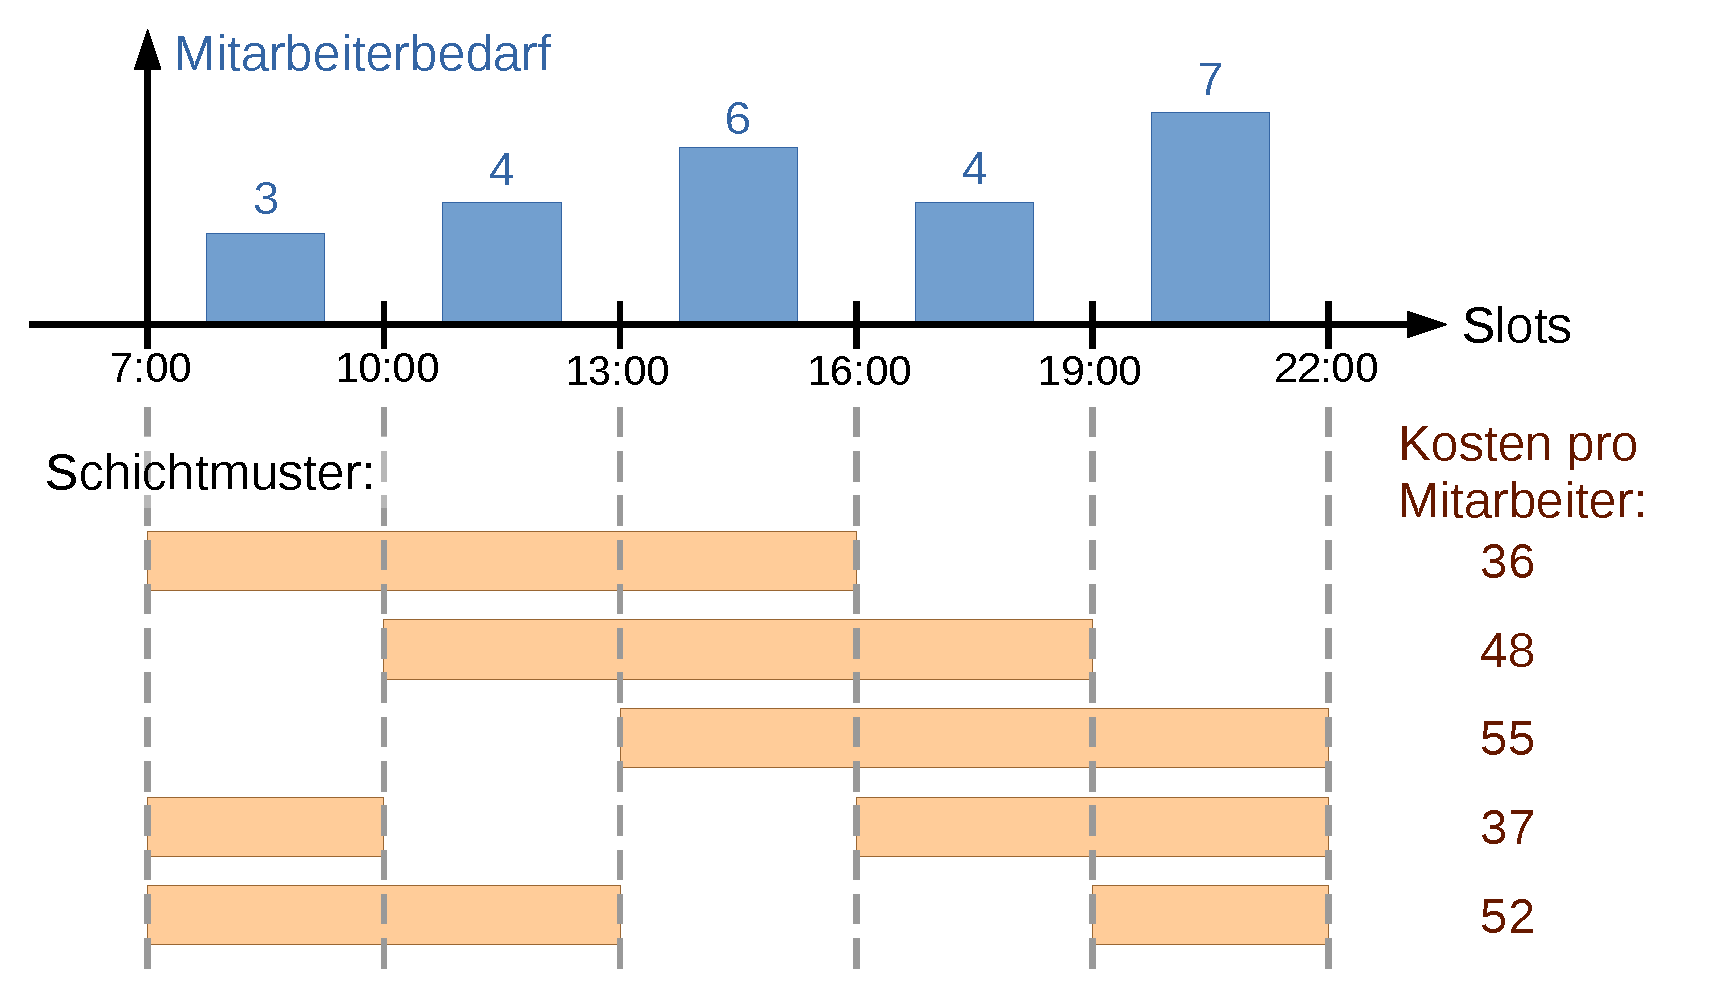
\includegraphics[width=\linewidth]{Bilder/Vindoo}
 \end{figure}
 {\footnotesize(vgl. Pinedo: Planning and Scheduling in Manufacturing and Services)}
\end{frame}

\begin{frame}
 \frametitle{Modell: Cyclic-Staffing-Problem}
 \begin{tabularx}{\linewidth}{lL}
  \multicolumn{2}{l}{\textbf{Indexmengen}:}\\
     $T$ & Menge der Zeitslots\\
     $S$ & Menge der Schichtmuster\\
  \multicolumn{2}{l}{\textbf{Parameter}:}\\
     $c_s$ & Kosten für Schichtmuster~$s\in S$\\
     $d_t$ & Bedarf in Zeitslot~$t\in T$\\
     $a_{ts}$ & Verfügbarkeit der Mitarbeiter aus Schichtmuster~$s\in S$ in Zeitslot~$t\in T$\\
  \multicolumn{2}{l}{\textbf{Entscheidungsvariablen}:}\\
     $x_s$ & Eingesetzte Mitarbeiter in Schichtmuster~$s\in S$\\[1ex]
  \multicolumn{2}{l}{\textbf{Modellbeschreibung}:}\\[1ex]
  \multicolumn{2}{l}{
      $
      \begin{array}{rllr}
	\min & \multicolumn{3}{l}{
		  \displaystyle\sum_{s\in S}c_s\cdot x_s
		}\\[3ex]
	s.t. & \displaystyle\sum_{s\in S} a_{ts}\cdot x_s \geq d_t & \quad\forall t\in T  & \mathrm{(I)}\\[.8ex]
	      & x_s \in\mathbb{Z}_0^+ & \quad\forall s\in S &\\
      \end{array}
      $
  }\\[1ex]
 \end{tabularx}
\end{frame}

\sectionframe[Optimierungs- ablauf in OPL]{Op\-ti\-mie\-rungs\-ab\-lauf in OPL}
\begin{frame}
 \frametitle{Optimierungsablauf in OPL}
 \begin{figure}
   \centering
   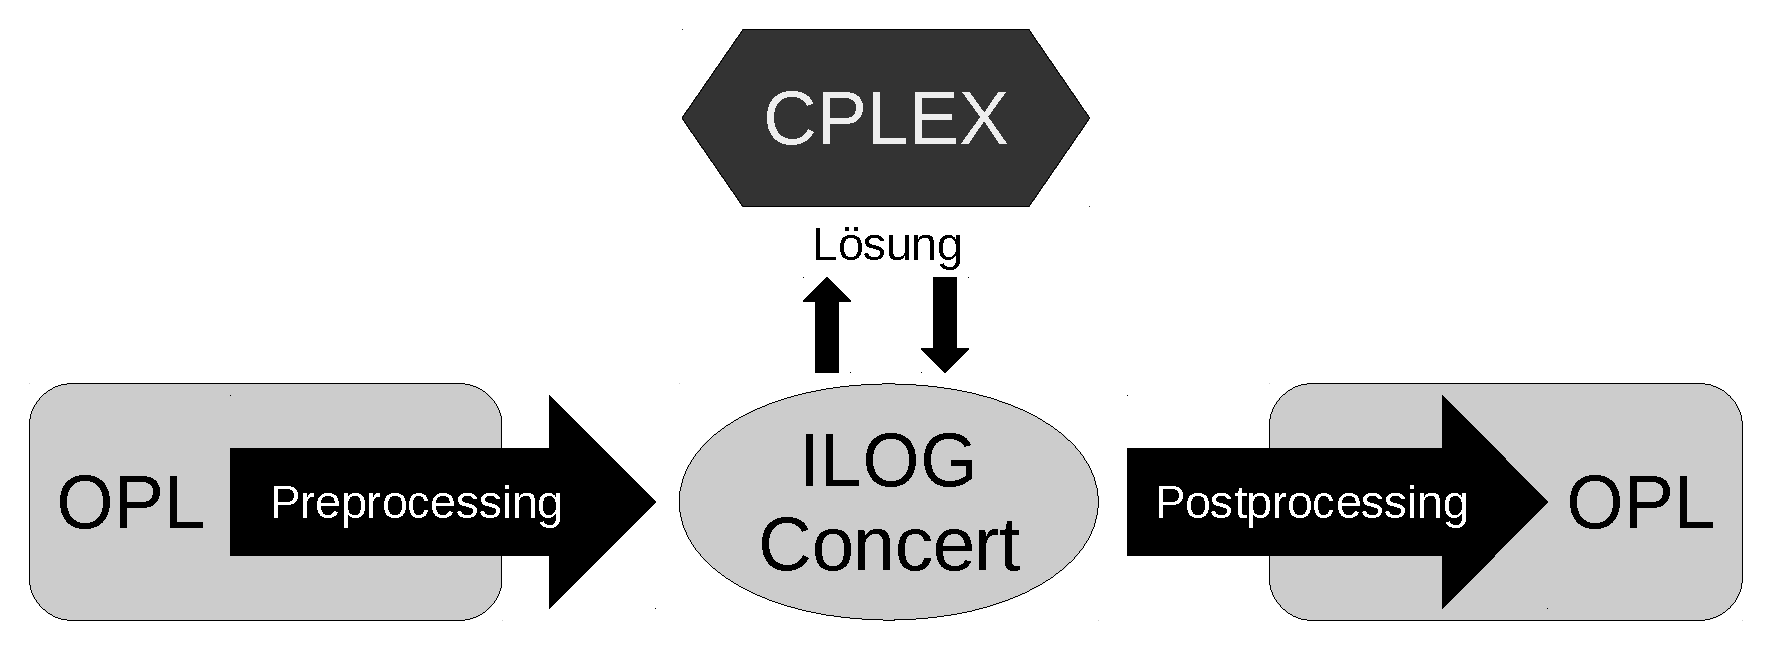
\includegraphics[width=\linewidth]{Bilder/OPL-Ablauf}
 \end{figure}
\end{frame}

